\begin{figure*}[t]
%\vspace{-1em}
%\subfigure[Figure A]{\label{fig:a}\includegraphics[width=60mm]{example-image-a}}
  \centering
 % \vspace{-1.5em}
  \subfloat{
    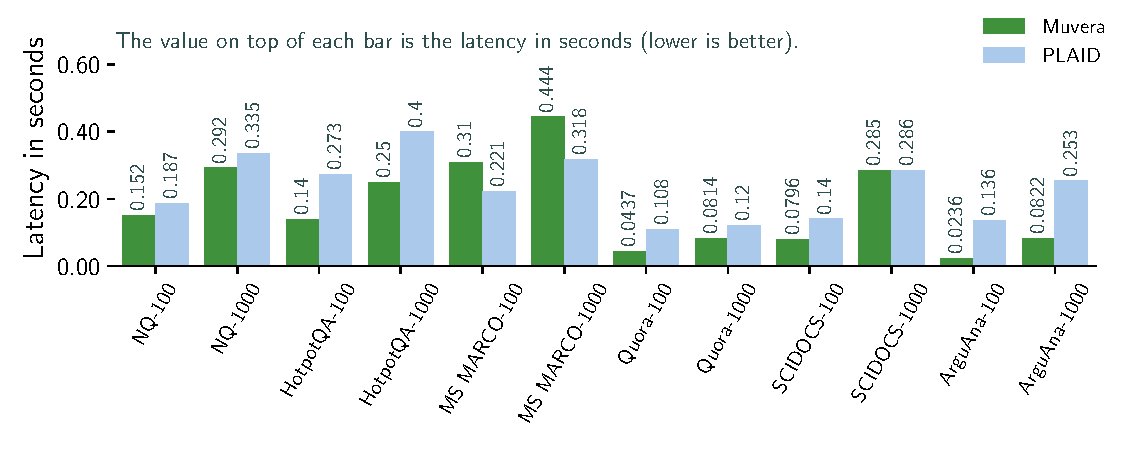
\includegraphics[width=.8\linewidth]{plots/latency-bar.pdf}} \\
 %  \vspace{-1.5em} 
  \subfloat{
    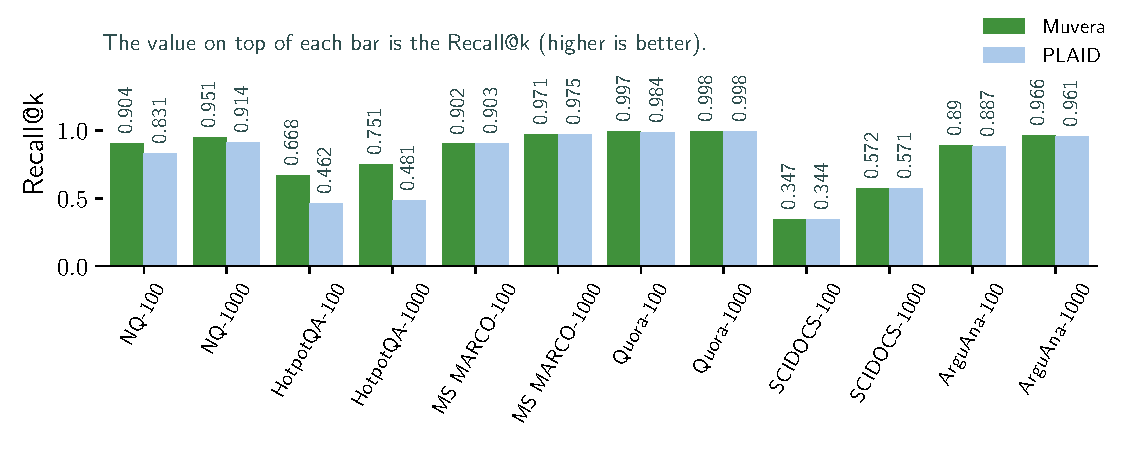
\includegraphics[width=.8\linewidth]{plots/recall-bar.pdf}}
%\vspace{-1em}
  \caption{\small Bar plots showing the latency and Recall@$k$ of \name{} vs PLAID on a subset of the BEIR datasets. The x-tick labels are formatted as dataset-$k$, i.e., optimizing for Recall@$k$ on the given dataset. \label{fig:vsplaid}}
\end{figure*}